\section{Architecture and Patterns}

\subsection{Application architecture}

The implementation of the project comprises of a single Java EE web application, running on top of a standard Java EE software stack as described in the Project Plan.\\

For the application to deliver on all of the functional requirements of the project in a robust, reliable and maintainable way, a proper architectural system design is needed, which should be followed throughout the implementation process.\\

Successful Java EE applications follow proven design patterns. Such patterns were researched, studied and prototyped to find the best solution for producing the kind of application we require.\\

After the successful development of a prototype, the following architecture has been chosen:

\begin{center}
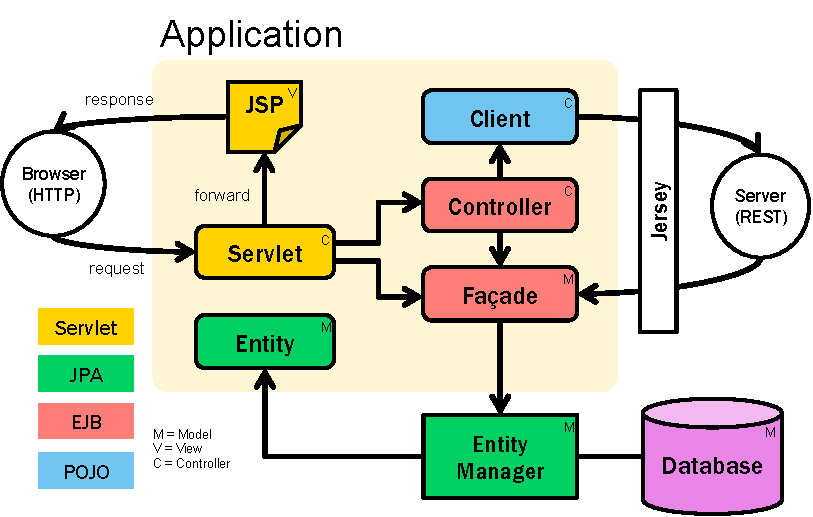
\includegraphics[scale=1]{img/architecture.pdf}  
\footnote{\textbf{JSP} JavaServer Pages}
\footnote{\textbf{JPA} Java Persistence API}
\footnote{\textbf{EJB} Enterprise Java Bean}
\footnote{\textbf{POJO} "Plain Old Java Object"}
\end{center}

The blocks represent modules in the system, and the thick lines show dependencies in the system.\\
The different colours of the modules indicate what kind of class they are.
Here is a brief overview of the concept:
\begin{itemize}
\item Data objects are defined as \textbf{Entity} classes. Entity objects are persisted to and retrieved from a database by the Java Persistence API.
\item The application retrieves and persists Entity objects via \textbf{Facade} classes.
\item Application logic is implemented in \textbf{Controllers}
\item User's browsers will invoke \textbf{Servlets} when they request a web page. Servlets respond to requests for data and actions. They request simple data transactions through Facades, and can defer more logical operations through Controllers.
\item The servlet's response gets forwarded to a related \textbf{JSP} page, which describes the view (the web page). When the JSP gets run, the data forwarded to it by the Servlet is inserted into the page in place of JSP tags.
\item Where data is required from multiple types of entities, facades can talk to other facades, and controllers can to other controllers where appropriate.
\item Other compatible servers can request data via a REST protocol, which special Service Facades handle. When this server wants to request data from another server, it does so through a Client class.
\end{itemize}

\clearpage
\subsection{Design Patterns}

\paragraph{Model-View-Controller}
Web applications by their very nature lean towards an MVC design paradigm. The view is the user's web browser, the controller is the application code and the model is the database. Not only this but MVC is a very robust and well proven pattern for designing applications. So MVC will be used throughout the design of the application.\\

To ensure MVC is correctly used, it should be very clear what packages, classes and other content does and doesn't do. The aim is to keep the Model, View and Controller implementation separate, so that, for example, model classes don't dictate how the data should look in a web page, that is the job of the view.

\paragraph{Facades}
The facade pattern will also be used as an extension of the Model to provide clean interfaces to the data. Facades will abstract away the details of persisting, retrieving and managing data from the database. By doing this, it prevents code related to database access from being spread across the application where access to data is required. Entity objects can be searched for, retrieved and persisted through single methods, rather than having JPA boilerplate code wherever entities need to be accessed.\\

Another advantage to using facades is that you can have multiple facades for the same set of data for different purposes. There will be facades for accessing data from within the application, and facades for accessing data over the inter-server REST protocol.

\paragraph{REST}
Representational State Transfer (ReST) will be used for inter-server communication with other group's servers. By using a set standard of API's, ReST allows easy access to data through standard HTTP methods. A client (whether it be a web browser or another application) can access data through URIs. By using standard HTTP methods, such as GET, POST and DELETE, this data can be accessed and manipulated without any special proprietary interfaces. The application will implement REST APIs through facades, where methods are invoked when a URI is requested, in a similar way that Servlets are instantiated when URLs are requested. Through the facade, data is returned, or processed depending on the method invoked. Entities will be serialised to JSON (Java Serialised Object Notation) object strings before being sent over REST. The application expects JSON object strings from other servers also, and they must be de-serialised back into entity objects.

\paragraph{EJB}
Controller and Facade classes are Enterprise Java Session Beans. This basically means that instances of those classes are handled by the Java EE runtime in Glassfish. Session Beans are not instantiated when they are needed, instead instances that are shared among multiple sessions are 'injected' into the dependant class. This reduces system resources, as there could be many sessions at once, instantiating the same class. Instead there is one instance for the application, shared among sessions.

\subsection{Required libraries}
The application should not require any libraries which are not available as part of a standard Java EE stack. The development environment, NetBeans, provides a full Java EE stack to develop from, including common libraries which may not be part of the Java EE distribution. There is one library which, while available with the standard NetBeans Java EE environment, needs to be explicitly included in the project. Other IDE's or distributions may not include this library, so it would need to be manually obtained and included in the build classpath.
\paragraph{Jersey 1.8}
Jersey is an open-source, production quality library for building RESTful web services in Java. It automatically handles the carriage of data over ReST to and from a Java EE application, and includes annotations which allow the invocation of methods when ReST resources are requested. It also includes \textbf{Jackson}, the most popular and probably best JSON serialiser/parser, and it automatically works with the ReST services provided in Jersey.\\

Jersey 1.8 is available in the latest version of NetBeans as an optional library with can be included in the project.\\

It can also be obtained from \textbf{jersey.java.net}